\section{Consistency of Common Concepts}
\label{chap:improvement:concpets}

\mnote{Alternative for consistency relations}
In our introduction in \autoref{chap:introduction}, we have motivated that models describing the same system share an overlap of information that leads to dependencies or in particular redundancies between the models.
Such dependencies need to be kept consistent to preserve a contradiction-free specification of the system.
We have made these dependencies explicit by means of consistency relations.
In the following, we discuss the alternative consideration of redundancies, as a special case of dependencies, by means of common concepts.
We therefore introduce an introductory example to be extended throughout the following considerations, explain the idea of \emph{\commonalities} and discuss in which cases it can reasonably be applied.


\subsection{Introductory Example}

\mnote{Example metamodels}
We employ a running example from the scenario introduced in \autoref{chap:introduction} involving \gls{PCM}~\cite{reussner2016a}, \gls{UML} and Java.
Consistency relations, as already introduced in the preceding chapters, comprise the common and mostly one-to-one mappings between \gls{UML} and Java, as well as the ones proposed by \textcite{langhammer2015a} to represent \gls{PCM} architecture models in Java code and also in \gls{UML} class models.

\begin{figure}
	\centering
	\newcommand{\vdistance}{7.5em}
\newcommand{\hdistance}{(18em+0.4*\difftoafiveimage)}
\newcommand{\classwidth}{5.5em}
\newcommand{\labeldistance}{0.2em}
\newcommand{\mmborder}{1.5em}


\begin{tikzpicture}

\pgfdeclarelayer{bg}
\pgfsetlayers{bg,main}


% METACLASSES

\umlclassvarwidth{java_class}{}{Class}{
name\\
}{\classwidth}  

\umlclassvarwidth[, below=\vdistance of java_class.center, anchor=center]{uml_class}{}{Class}{
name\\
}{\classwidth} 

\umlclassvarwidth[, below left=0.5*\vdistance and \hdistance of java_class.center, anchor=center]{pcm_component}{}{Component}{
name\\
}{\classwidth} 


% METAMODELS

\coordinate (java_label_coordinate) at ([yshift=\labeldistance]java_class.north);
\node[mmlabel, anchor=south] (java_label) at (java_label_coordinate) {Java};

\coordinate (uml_label_coordinate) at ([yshift=-\labeldistance]uml_class.south);
\node[mmlabel, anchor=north] (java_label) at (uml_label_coordinate) {\acrshort{UML}};

\coordinate (pcm_label_coordinate) at ([xshift=-7*\labeldistance]pcm_component.west);
\node[mmlabel, right=6*\labeldistance of pcm_label_coordinate, anchor=east] (pcm_label) {\acrshort{PCM}};

\begin{pgfonlayer}{bg}
    \node[mmbg, fit=(java_class)(java_label_coordinate), inner sep=\mmborder] (java) {};
    \node[mmbg, fit=(uml_class)(uml_label_coordinate), inner sep=\mmborder] (uml) {};
    \node[mmbg, fit=(pcm_component)(pcm_label_coordinate), inner sep=\mmborder] (pcm) {};
\end{pgfonlayer}


% CONSISTENCY RELATIONS

\draw[directed consistency relation] (pcm_component) |- node[pos=0, above left] {$\mathvariable{co}$} node[above, pos=0.65, align=center] {$\setted{\tupled{\mathvariable{co}, \mathvariable{cl}} \mid \mathvariable{cl.name} = \mathvariable{co.name} + "\mathvariable{Impl}"}$} node[pos=1, below left] {$\mathvariable{cl}$} (java_class);
\draw[consistency relation] (java_class) -- node[pos=0, below right] {$\mathvariable{jcl}$} node[left] {$\setted{\tupled{\mathvariable{jcl}, \mathvariable{ucl}} \mid \mathvariable{jcl.name} = \mathvariable{ucl.name}}$} node[pos=1, above right] {$\mathvariable{ucl}$} (uml_class);
\draw[directed consistency relation] (pcm_component) |- node[pos=0, below left] {$\mathvariable{co}$} node[below, pos=0.65, align=center] {$\setted{\tupled{\mathvariable{co}, \mathvariable{cl}} \mid \mathvariable{cl.name} = \mathvariable{co.name} + "\mathvariable{Impl}"}$} node[pos=1, above left] {$\mathvariable{cl}$} (uml_class);

\end{tikzpicture}

	\caption[Consistency relations for extracts of Java, UML and PCM]{Simple metamodel extracts for Java, UML and \gls{PCM} and consistency relations between them. Adapted from \owncite[Fig.~1]{klare2019models}.}
	\label{fig:improvement:running_example}
\end{figure}

\mnote{Example relations}
In the following, we start with limited subsets of the metamodels, namely the one-to-one mapping between components in \gls{PCM} and classes in Java, whereby each component is mapped to a class but not vice versa, as depicted in \autoref{fig:improvement:running_example}.
Consistency relations require the existence of a class in \gls{UML} and Java for each \gls{PCM} component with the same name appended by an \enquote{Impl} suffix (cf.~\cite{langhammer2015a}) by an according unidirectional consistency relation, and a \gls{UML} class for each Java class with the same name and vice versa.
We extend this example through the following sections to explain the introduced concepts.


\subsection{Explicit Commonalities}
\label{chap:improvement:concepts:explicit}

\mnote{Common concepts}
In the given example, classes are redundantly represented in Java and \gls{UML}.
This requires them to be kept consistent, for example, by means of an according consistency relation.
As an alternative, redundant classes in a Java and a \gls{UML} model can also be considered representations of a \emph{common concept}, more precisely the common concept of a class in general object-oriented design.
Thus, rather than expressing this redundancy implicitly by means of a consistency relation and transformation that preserves consistency to it, we propose to make the common concept explicit in an according metamodel and descriptions of how this concept \emph{manifests} in Java and \gls{UML}.
Then, instead of saying that each \gls{UML} class should corresponding to a Java class and vice versa, we would say that classes in \gls{UML} and Java are both representations of the same concept of a class in object-oriented design.

\begin{figure}
    \centering
    \newcommand{\vdistance}{7.5em}
\newcommand{\hdistance}{15em}
\newcommand{\classwidth}{5.5em}
\newcommand{\labeldistance}{1.2em}
\newcommand{\labelshift}{0.3*\classwidth}
\newcommand{\mmborder}{1em}

\begin{tikzpicture}

\pgfdeclarelayer{bg}
\pgfsetlayers{bg,main}


% METACLASSES

\umlclassvarwidth{java_class}{}{Class}{
name\\
}{\classwidth}  

\umlclassvarwidth[, right=\hdistance of java_class.north, anchor=north]{uml_class}{}{Class}{
name\\
}{\classwidth} 

\umlclassvarwidth[, above right=\vdistance and 0.5*\hdistance of java_class.north, anchor=north]{oo_class}{}{Class\vphantom{p}}{
name\\
}{\classwidth} 


% METAMODELS

\coordinate (java_label_coordinate) at ([yshift=\labeldistance]java_class.north west);
\node[mmlabel, anchor=west] (java_label) at (java_label_coordinate) {Java};

\coordinate (uml_label_coordinate) at ([xshift=\labelshift,yshift=\labeldistance]uml_class.north);
\node[mmlabel, anchor=center] (java_label) at (uml_label_coordinate) {UML};

\coordinate (oo_label_coordinate) at ([yshift=\labeldistance]oo_class.north);
\node[mmlabel, anchor=center] (oo_label) at (oo_label_coordinate) {Object-oriented Design};

\begin{pgfonlayer}{bg}
    \node[mmbg, fit=(java_class)(java_label_coordinate), inner sep=\mmborder] (java) {};
    \node[mmbg, fit=(uml_class)(uml_label_coordinate), inner sep=\mmborder] (uml) {};
    \node[conceptmmbg, minimum width=11.5em, fit=(oo_class)(oo_label_coordinate), inner sep=\mmborder] (oo) {};
\end{pgfonlayer}


% CONSISTENCY RELATIONS

\draw[manifests relation] (oo_class) -- node[manifests relation, above, sloped] {\manifestslabel} (java_class);
\draw[manifests relation] (oo_class) -- node[manifests relation, above, sloped] {\manifestslabel} (uml_class);

\end{tikzpicture}

    \caption[One \commonality example for object-oriented design]{\Conceptmetamodel for object-oriented design with a \texttt{Class} \commonality and its relations to the \concretemetamodels \gls{UML} and Java. Adapted from \owncite[Fig.~2]{klare2019models}.}
    \label{fig:improvement:one_commonality_example}
\end{figure}

\mnote{Concepts and their relations}
We denote the actual metamodels that developers instantiate and want to keep consistent as \emph{\concretemetamodels}, whereas we denote metamodels that describe the concepts such \concretemetamodels have in common as \emph{\conceptmetamodels}.
\autoref{fig:improvement:one_commonality_example} depicts the \concretemetamodels \gls{UML} and Java with their representations of classes.
In addition, it contains a \conceptmetamodel for object-oriented design, which contains the common concept of a class, shared by \gls{UML} and Java.
We denote a single common concept, such as a class, as a \emph{\commonality}.
Further \commonalities in object-oriented design would be interfaces or methods.
In general, a \commonality can be considered a \metaclass with the specific semantics of describing the commonalities between elements of \concretemetamodels.
We say that an element in a \concretemetamodel such as classes in \gls{UML} and Java are a \emph{manifestation} of a common concept.
The relation of a \commonality to these manifestations is denoted by a manifestation (\emph{«manifests»}) relation.
In the given example, the relations would especially define that each class manifestation conforms to a common class concept having the same name and vice versa, as depicted in the consistency relations defined in \autoref{fig:improvement:running_example}.

\mnote{Specification effort}
In fact, these manifestation relations can be considered transformations again.
Thus, in a first place the representation of common concepts in terms of explicit \commonalities introduces further effort, because it requires the definition of one metamodel and two transformations instead of a single transformation relating the \metaclasses directly.
This drawback is, however, reduced by several benefits, which we discuss in \autoref{chap:improvement:benefits}, in particular mitigating trade-offs between correctness and reusability and improving comprehensibility.
Finally, this way of specifying consistency can even reduce specification effort due to better scalability when adding further \concretemetamodels to keep consistent.
For example, if another object-oriented language such as \cplusplus shall be kept consistent, no matter whether only with \gls{UML} or indeed even with Java, only the manifestation relation from \commonalities in the object-oriented \conceptmetamodel to \cplusplus has to be added, potentially along with some extensions of the \conceptmetamodel for information shared between \cplusplus and \gls{UML} that was not already shared between Java and \gls{UML}.
This already reduces the effort in comparison to defining both relations between \cplusplus and \gls{UML}, as well as between \cplusplus and Java.

\begin{figure}
    \centering
    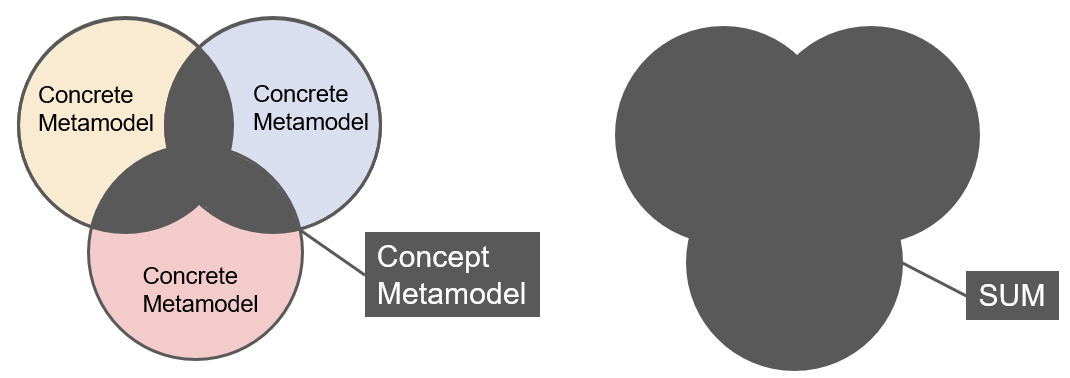
\includegraphics[width=\textwidth]{figures/quality/improvement/commonalities_and_sums.png}
    \caption[Commonalities compared to \acrlongpl{SUM}]{Sketch for the scope of contents of \conceptmetamodels in comparison to those of \glspl{SUM}.}
    \label{fig:improvement:commonalities_and_sums}
\end{figure}

\mnote{Size of concept metamodels}
In general, a \conceptmetamodel has to contain \commonalities for all redundancies between the \concretemetamodels to keep consistent.
In a mathematical sense, this can be considered as the union of all pairwise intersections of the \concretemetamodels.
It can, however, not be precisely expressed as such, because elements may be similarly represented in the \concretemetamodels, but they are not the same.
One manifestation of the same \commonality may contain more or different information than the others, or it may encode information differently, such as using different units.
This already illustrates the essential difference to approaches in which one central model unifies all information about a system, called a \gls{SUM}~\cite{atkinson2010a}, from which the information represented in models used by different tools is derived by projection.
Such a \gls{SUM} can be seen as the union of all \concretemetamodels, in contrast to the union of the pairwise intersections represented by \concretemetamodels.
We illustrate these relations in \autoref{fig:improvement:commonalities_and_sums}.


\subsection{Consistency Specification Types}
\label{chap:improvement:concepts:specification}

\mnote{Descriptive and normative specifications}
In \autoref{chap:networks:notions:normative_descriptive}, we have discussed the distinction between descriptive and normative specifications of consistency, which can be summarized as follows:
\begin{properdescription}
    \item[Descriptive Specification:] Descriptive specifications describe consistency relations that are \enquote{naturally} given when two metamodels represent common \emph{concepts} redundantly or at least with common or dependent properties. 
    In that case, a notion of consistency already exists, either formally or informally, to which the given specification must conform.
    This is, for example, the case for \gls{UML} class models and Java realizing object-oriented design.
    \item[Normative Specification:] Normative specifications prescribe consistency for metamodels for which no existing or common notion for consistency exists.
    This is especially the case if metamodels represent different abstractions or domains of a system, which have no implicit relations and for which different possibilities to relate them exist, such as an \gls{ADL} like \gls{PCM} and Java.
\end{properdescription}
While descriptive consistency relations between two metamodels are usually definite, such as those for object-oriented design between \gls{UML} and Java, normative consistency relations may vary depending on the project context.
For example, several possible relations can be defined between an \gls{ADL} such as \gls{PCM} and object-oriented design, for example the realization of each component as a class, as a bean in \glspl{EJB}, or as a complete project~\cite{langhammer2017a}.

\mnote{Suitability for descriptive specification}
Describing consistency by means of \commonalities and \conceptmetamodels especially promises to be useful for descriptive consistency specifications, where a \enquote{natural} relation existing due to elements representing common concepts.
It can, however, also be used to normatively define commonalities in terms of a normative specification.
A component \commonality can, for example, define that a component manifests as a component in \gls{PCM} and as a class in \gls{UML} and Java, or, more generally, in an object-oriented design \conceptmetamodel.
The will, however, unlikely fit well for rather complex dependencies, such as a consistency relation between performance requirements and the implementation, which require the implementation to fulfill some kind of performance requirement.
In such a case, the complexity is in the specification of the consistency relation anyway, which would have to be replicated when defining a \commonality between performance requirement and implementation.
Finally, this conforms to our distinction of structural and behavioral consistency relations given in \autoref{chap:networks:notions:types}, in which the \commonalities fit well into structural relations.
We have also stated to focus on such structural relations for the context of this thesis.

\mnote{Generalization}
In the following, we do not distinguish whether \commonalities are defined for common concepts that exist naturally, or for those which are prescribed by the definition of \conceptmetamodels and their \commonalities.
We will see that even for normative specifications \commonalities can be reasonably defined.
In \autoref{chap:improvement:application}, we will, however, also discuss how to combine ordinary transformations with the idea of \conceptmetamodels.


% \begin{copiedFrom}{VoSE}

% \section*{Running Example}

% We use a running example throughout the paper to explain the \commonalities idea.
% It relies on three metamodels: UML class models, Java code, whose grammar definition can be treated as a metamodel~\cite{heidenreich2010a}, and the \gls{PCM}~\cite{reussner2016a}, a component-based architecture description language.
% The consistency relations between Java and UML class models are mostly one-to-one mappings, as they provide the same concepts of object-oriented design. %provide redundant representations of the same concepts, so the consistency relations between them define mostly one-to-one mappings.
% Consistency relations between \gls{PCM} and Java were proposed by \textcite{langhammer2015a}.
% For this paper, only the one-to-one mapping between components in \gls{PCM} and classes in Java---or generally all object-oriented languages---are relevant, whereby each component is mapped to a class but not vice versa.

% For the examples in this paper, a minimalist subset of those metamodels, depicted in \autoref{fig:improvement:running_example}, is sufficient.
% It only comprises classes in UML and Java and components in \gls{PCM}, which all have a name.
% The name shall be equal between corresponding classes in UML and Java, whereas the classes realizing a component shall have the same name as the component, complemented by an \enquote{Impl} suffix (cf.~\cite{langhammer2015a}).
% With state-of-the-art techniques, those constraints could be implemented as relations in declarative or as enforcing routines in imperative transformation languages.

% \begin{figure}
% 	\centering
% 	\newcommand{\vdistance}{7.5em}
\newcommand{\hdistance}{(18em+0.4*\difftoafiveimage)}
\newcommand{\classwidth}{5.5em}
\newcommand{\labeldistance}{0.2em}
\newcommand{\mmborder}{1.5em}


\begin{tikzpicture}

\pgfdeclarelayer{bg}
\pgfsetlayers{bg,main}


% METACLASSES

\umlclassvarwidth{java_class}{}{Class}{
name\\
}{\classwidth}  

\umlclassvarwidth[, below=\vdistance of java_class.center, anchor=center]{uml_class}{}{Class}{
name\\
}{\classwidth} 

\umlclassvarwidth[, below left=0.5*\vdistance and \hdistance of java_class.center, anchor=center]{pcm_component}{}{Component}{
name\\
}{\classwidth} 


% METAMODELS

\coordinate (java_label_coordinate) at ([yshift=\labeldistance]java_class.north);
\node[mmlabel, anchor=south] (java_label) at (java_label_coordinate) {Java};

\coordinate (uml_label_coordinate) at ([yshift=-\labeldistance]uml_class.south);
\node[mmlabel, anchor=north] (java_label) at (uml_label_coordinate) {\acrshort{UML}};

\coordinate (pcm_label_coordinate) at ([xshift=-7*\labeldistance]pcm_component.west);
\node[mmlabel, right=6*\labeldistance of pcm_label_coordinate, anchor=east] (pcm_label) {\acrshort{PCM}};

\begin{pgfonlayer}{bg}
    \node[mmbg, fit=(java_class)(java_label_coordinate), inner sep=\mmborder] (java) {};
    \node[mmbg, fit=(uml_class)(uml_label_coordinate), inner sep=\mmborder] (uml) {};
    \node[mmbg, fit=(pcm_component)(pcm_label_coordinate), inner sep=\mmborder] (pcm) {};
\end{pgfonlayer}


% CONSISTENCY RELATIONS

\draw[directed consistency relation] (pcm_component) |- node[pos=0, above left] {$\mathvariable{co}$} node[above, pos=0.65, align=center] {$\setted{\tupled{\mathvariable{co}, \mathvariable{cl}} \mid \mathvariable{cl.name} = \mathvariable{co.name} + "\mathvariable{Impl}"}$} node[pos=1, below left] {$\mathvariable{cl}$} (java_class);
\draw[consistency relation] (java_class) -- node[pos=0, below right] {$\mathvariable{jcl}$} node[left] {$\setted{\tupled{\mathvariable{jcl}, \mathvariable{ucl}} \mid \mathvariable{jcl.name} = \mathvariable{ucl.name}}$} node[pos=1, above right] {$\mathvariable{ucl}$} (uml_class);
\draw[directed consistency relation] (pcm_component) |- node[pos=0, below left] {$\mathvariable{co}$} node[below, pos=0.65, align=center] {$\setted{\tupled{\mathvariable{co}, \mathvariable{cl}} \mid \mathvariable{cl.name} = \mathvariable{co.name} + "\mathvariable{Impl}"}$} node[pos=1, above left] {$\mathvariable{cl}$} (uml_class);

\end{tikzpicture}

% 	\caption[Consistency relations for extracts of Java, UML and PCM]{Simple metamodel extracts for Java, UML and \gls{PCM} and consistency relations between them.}
% 	\label{fig:improvement:running_example}
% \end{figure}

% In this paper, we consider metamodels that conform to the \gls{EMOF} standard~\cite{mof}.
% Such metamodels consist of classes, which we denote as \emph{\metaclasses} to avoid confusion with classes in exemplary metamodels such as Java and UML.
% \Metaclasses can in turn contain attributes and associations to other classes, which may be containments.


% \subsection*{Making Common Concepts Explicit}

% The redundancies between different metamodels are an expression of common concepts that are represented redundantly.
% We already gave the example of a class in UML and Java, which are different representations of the common concept of a class in general object-oriented design.
% We propose to make common concepts explicit rather than encoding them into the rules of a transformation.
% This can be achieved by creating a \emph{\conceptmetamodel}, which defines those common concepts, and specifying the relations between the \conceptmetamodel and the existing metamodels.
% We refer to the existing metamodels as \emph{\concretemetamodels}.
% The relation specifications can be used to derive transformations between the \concretemetamodels and the \conceptmetamodel.

% \autoref{fig:quality:commonalities_example} shows the \metaclasses for a \texttt{Class} as extracts of the \concretemetamodels for UML and Java and the \metaclass for the common concept of a \texttt{Class} in the \conceptmetamodel for object-oriented design.
% We denote a single common concept as a \emph{\commonality}.
% Further \commonalities in object-oriented design could, for example, be interfaces or methods.
% The relation between the \texttt{Class} \commonality and its realizations in the \concretemetamodels are shown by a \emph{«manifests»} relation.
% %Such a relation can be defined in a transformation.
% In our simplified example, the relation would especially define that the names of the classes have to be equal. %an equality relationship.

% \begin{figure}
%     \centering
%     \newcommand{\vdistance}{7.5em}
\newcommand{\hdistance}{11em}
\newcommand{\classwidth}{5.5em}
\newcommand{\labeldistance}{1.2em}
\newcommand{\labelshift}{0.3*\classwidth}
\newcommand{\representstext}{\emph{«manifests»}}
\newcommand{\mmborder}{1em}

\begin{tikzpicture}

\pgfdeclarelayer{bg}
\pgfsetlayers{bg,main}


% METACLASSES

\umlclassvarwidth{java_class}{}{Class}{
name\\
}{\classwidth}  

\umlclassvarwidth[, right=\hdistance of java_class.north, anchor=north]{uml_class}{}{Class}{
name\\
}{\classwidth} 

\umlclassvarwidth[, above right=\vdistance and 0.5*\hdistance of java_class.north, anchor=north]{oo_class}{}{Class\vphantom{p}}{
name\\
}{\classwidth} 


% METAMODELS

\coordinate (java_label_coordinate) at ([xshift=-\labelshift,yshift=\labeldistance]java_class.north);
\node[mmlabel, anchor=center] (java_label) at (java_label_coordinate) {Java};

\coordinate (uml_label_coordinate) at ([xshift=\labelshift,yshift=\labeldistance]uml_class.north);
\node[mmlabel, anchor=center] (java_label) at (uml_label_coordinate) {UML};

\coordinate (oo_label_coordinate) at ([yshift=\labeldistance]oo_class.north);
\node[mmlabel, anchor=center] (oo_label) at (oo_label_coordinate) {Object-oriented Design};

\begin{pgfonlayer}{bg}
    \node[mmbg, fit=(java_class)(java_label_coordinate), inner sep=\mmborder] (java) {};
    \node[mmbg, fit=(uml_class)(uml_label_coordinate), inner sep=\mmborder] (uml) {};
    \node[conceptmmbg, minimum width=11.5em, fit=(oo_class)(oo_label_coordinate), inner sep=\mmborder] (oo) {};
\end{pgfonlayer}


% CONSISTENCY RELATIONS

\draw[consistencyrel, <-] (java_class) -- node[above, sloped] {\representstext} (oo_class);
\draw[consistencyrel, <-] (uml_class) -- node[above, sloped] {\representstext} (oo_class);

\end{tikzpicture}

%     \caption[Concept metamodel for object-oriented design]{\Conceptmetamodel for object-oriented design with a \texttt{Class} \commonality and its relations to UML and Java.}
%     \label{fig:quality:commonalities_example}
% \end{figure}

% When another \concretemetamodel that represents the same concepts shall be added, it is only necessary to define its relation to the \conceptmetamodel.
% For example, adding \cplusplus as another metamodel representing object-oriented design would require the definition of the relation between the \texttt{Class} \commonality in object-oriented design and its representation in \cplusplus.
% Adding an additional metamodel may require the \conceptmetamodel to be extended by \commonalities that were not relevant for the already considered metamodels.
% In general, a \conceptmetamodel has to contain \commonalities for redundancies in all \concretemetamodels, which---mathematically speaking---can be expressed as the union of all pairwise intersections of the \concretemetamodels.

% Short description of the Commonalities concept and application to example (UML and Java classes, could e.g. be extended by C++)
% Necessary artifacts: the Commonalities metamodel and the transformations.
% But: one can define a language to specify the Commonalities metamodel together with a specification of how the elements and properties manifest in the concrete metamodels, which we will explain in more detail in \autoref{sec:language}.
% Introduce terms: \emph{Commonality} (metamodel with common concepts), concrete metamodel (a metamodel that is accessed by a user) and \emph{Manifestation} (the concrete metamodels that realize a Commonality).
% \end{copiedFrom} % VoSE


% \begin{copiedFrom}{DocSym}

% \section*{Making Common Concepts Explicit} 

% \subsection{Approach
%     \pgsize{1 p.}
%     \dl{16.06.2017}
%     \complete{0}}

%\todoConference{A description of the proposed solution and which other work (e.g., methods or tools) it depends on.}
%\todoHeiko{One Solution: Add additional models. Already proposed by Stevens, but just to solve constraints. Here, we make overlaps explicit}
%\todo{Referenz zu Aussage von Stevens hinzufügen}
%\todoHeiko{Discuss necessity to provide orthogonal concept metamodels}

%\todoHeiko{Why ''virtual``? Because they are transparent to the user and nothing he has to deal with}
%\todo{Referenz auf Grafik und Optimalfall davon erklären}
% Based on the decomposition of consistency relations, we propose another approach to achieve a tree structure of transformations, which inherently optimizes \emph{modularity}.
%In the following, we propose another solution option to achieve a tree structure of consistency relations, next to decomposing consistency relations into independent subsets.
%This approach called \emph{\acp{CMM}} ensures consistency between specifications inherently given by the tree structure, but also optimizes modularity, so that an arbitrary subset of the metamodels can be used.
%It also reuses the concepts for decomposing consistency relations.
% In \autoref{sec:Introduction}, we discussed reasons for specifying consistency using binary transformations instead of defining multiary relations.
% Nevertheless, as discussed in the previous section, trade-off decisions regarding the identified challenges have to made with that approach.
% Therefore, we propose an approach called \emph{\acp{CMM}} for a certain kind of relations that addresses all those identified challenges.
% The idea bases on the insight that we can distinguish two kinds of consistency relations:
% \begin{description}[leftmargin=\parindent]
%     \item[Descriptive consistency relations] are \enquote{naturally} given when two metamodels represent common \emph{concepts} %with common properties
%     redundantly or at least with dependent properties. This is, for example, the case for \gls{UML} class models and Java realizing \gls{OO}. %, and for \ac{UML} component models and \ac{PCM} models realizing a component concept.
%     %They have to be expressed by transformations in a way that they describe the underlying consistency relations.
%     \item[Normative consistency relations] prescribe consistency and %are induced by transformations and that 
%     do not exist \enquote{naturally}. This is especially the case if metamodels represent different abstractions or domains of a system, which have no implicit relation, such as an \gls{ADL} and Java. % in our example.
% \end{description}

% While descriptive consistency relations between two metamodels are usually definite, such as those between \gls{OO} design in \gls{UML} and Java, normative consistency relations may vary depending on the project context.
% For example, several possible relations can be defined between an \gls{ADL} and \gls{OO} design, for example the realization of each component as a class or as a complete project~\cite{langhammer2017a}.
%$For example, the relation between \ac{OO} design in \ac{UML} and Java will usually be definite and not depend on the context, whereas there may be several possible relations between an \ac{ADL} and OO-design.
%Depending on the context, a component could be realized by a class or a complete project, and a class realizing an architectural component may be placed anywhere or in a specific package, as discussed by \textcite{langhammer2017a}.

% Transformations for descriptive consistency relations implicitly encode %the preservation of consistency between 
% the common concepts.
% %Descriptive consistency relations base on the fact that different metamodels represent similar or equal concepts.
% %In consequence, transformations are supposed to define the preservation of consistency between those common concepts.
% %Instead of implicitly encoding those common concepts in transformations, 
% Instead, we propose to make these common concepts explicit in so-called \emph{\glspl{CMM}} and define relations between them and the concrete metamodels.
% We illustrate this in \autoref{fig:quality:concept_metamodel_integration}.
% The descriptive consistency relation \ref{fig:quality:concept_metamodel_integration:R1} is converted into a \gls{CMM} for the metamodels \ref{fig:quality:concept_metamodel_integration:A} and \ref{fig:quality:concept_metamodel_integration:B} with new relations \ref{fig:quality:concept_metamodel_integration:R4} and \ref{fig:quality:concept_metamodel_integration:R5} between the concrete metamodels and the \gls{CMM}.
% The existing normative consistency relations \ref{fig:quality:concept_metamodel_integration} and \ref{fig:quality:concept_metamodel_integration:R3} to metamodel \ref{fig:quality:concept_metamodel_integration:C} are replaced by a new relation \ref{fig:quality:concept_metamodel_integration:R6} to the \gls{CMM}. % to the metamodel \ref{fig:concept:C}.
% The \gls{CMM} and its consistency relations have to be appropriately defined to replace the original ones, as depicted in \autoref{fig:quality:concept_metamodel_integration}. %, have to be fulfilled by appropriately defining the \ac{CMM}.
% It will be part of our research to figure out how to define such a \gls{CMM}, so that it can also be combined with other metamodels. %, without estimating the additional information that may be necessary in the \ac{CMM} a-priori.
% While it basically has to contain the common concepts of the metamodels sharing a descriptive consistency relations, it may also need to contain additional information depending on consistency relations to other metamodels, which are not known a-priori.

% \begin{figure}
%     \centering
%     \newcommand{\mmdistance}{8em}

\begin{tikzpicture}[
    mm/.style={draw, circle, fill=lightgray, inner sep=0.25em},
    consistencyrel/.style={latex-latex,dashed}]


\node[mm] (original_left) {\mylabel{fig:quality:concept_metamodel_integration:A}{$A$}};
\node[mm, right=\mmdistance of original_left.center, anchor=center] (original_middle) {\mylabel{fig:quality:concept_metamodel_integration:B}{$B$}};
\node[mm, right=\mmdistance of original_middle.center, anchor=center] (original_right) {\mylabel{fig:quality:concept_metamodel_integration:C}{$C$}};

\draw[consistencyrel] (original_left) -- node[above] {\mylabel{fig:quality:concept_metamodel_integration:R1}{$R_1$}} node[below] {\textit{descriptive}} (original_middle);
\draw[consistencyrel] (original_middle) to[bend left=30] node[above] {\mylabel{fig:quality:concept_metamodel_integration:R2}{$R_2$}} node[below=0.2em] {\textit{normative}} (original_right);
\draw[consistencyrel] (original_left) to[bend right=40] node[above] {\mylabel{fig:quality:concept_metamodel_integration:R3}{$R_3$}} node[below] {\textit{normative}} (original_right);


\node[mm, fill=gray!10, above right=0.55*\mmdistance and 0.5*\mmdistance of original_left.center, anchor=center, align=center] (concept) {$AB-$\\$CMM$};

\draw[consistencyrel, color=gray] (original_left) -- node[above left=-0.3em and 0.5em] {\mylabel{fig:quality:concept_metamodel_integration:R4}{$R_4$}} (concept);
\draw[consistencyrel, color=gray] (original_middle) -- node[above right=-0.3em and 0.3em] {\mylabel{fig:quality:concept_metamodel_integration:R5}{$R_5$}} (concept);
\draw[consistencyrel, color=gray] (original_right) to[bend right=30] node[pos=0.6, below left] {\mylabel{fig:quality:concept_metamodel_integration:R6}{$R_6$}} (concept);



\node[right=2.5*\mmdistance of concept.north, anchor=north east, align=left] { 
$R_1 \concat R_2 \neq (R_1 \concat R_2) \cap R_3 \neq R_3$
};

\node[below right=2em and 2.5*\mmdistance of concept.north, anchor=north east, align=left] {
$R_4 \concat R_5 = R_1$\\
$R_4 \concat R_6 = R_3$\\
$R_5 \concat R_6 = R_2$\\
};


\end{tikzpicture}
%     \caption{Definition of a concept metamodel}
%     \label{fig:quality:concept_metamodel_integration}
%     \todo{We can use this for showing how to integrate commonalities with ordinary direct relations, maybe there should be a section about that.}
% \end{figure}

%%%As one concrete example, instead of specifying transformations between \ac{OO} design in \ac{UML} and Java, an OO-\ac{CMM}, with concepts like classes, inheritance and so on, and the relations of \ac{UML} and Java to this \ac{CMM} could be defined.
% These concept metamodels can be seen as additional metamodels 
% of metamodels having inherent consistency relations explicit within a \ac{VOMM} and to define a mapping between concrete metamodels and \acp{VOMM}. We claim that prescribed consistency is actually not specific for concrete metamodels, but for concepts as represented by our \acp{VOMM}, which means that metamodels with prescribed consistency relations can be kept consistent by specifying consistency preservation between their \acp{VOMM}. In our example, this means that consistency relations between \ac{PCM} and Java should be expressed as relations between OO and component concept. 

%%%%% CBSE-EXAMPLE REMOVED!
% In \autoref{fig:cmm_example}, we illustrate the usage of such \acp{CMM} to define an OO-concept and a concept for component-based architecture descriptions, relating component models of \ac{UML} and the \acf{PCM} to.
% Relations between those \acp{CMM} can again be defined using other \acp{CMM}, or by defining ordinary transformations between them. 
% We discuss the impact of that decision in the following.

% \begin{figure}
%     \vspace{-0.7em}
%     \begin{center}
%         \input{figures/cmm_example.tex}
%     \end{center}
%     \vspace{-0.7em}
%     \caption{Exemplary \acp{CMM} and their consistency relations}
%     \label{fig:cmm_example}
% \end{figure}

%\todoHeiko{Das mit der Baumstruktur ist ein Knackpunkt. Kommt der gut genug rüber?}
% To avoid the drawbacks of transitive transformation execution between \acp{VOMM}, it is necessary that only one propagation path between two metamodels exists. This requires to define \ac{VOMM} relations in a way such that they induce an an acyclic graph by also extracting common concepts of \acp{VOMM} in another \ac{VOMM}. 
%In the example, the component \ac{VOMM} could be seen as an abstracted concept of the OO \ac{VOMM}. 
% It will be part of our research to identify if such an ordering of concepts can be achieved in different case studies.

%%% REMOVED THE FOLLOWING, AS NOT A RELEVANT "DRAWBACK"
%Such \acp{CMM} are technically similar to introducing new metamodels and defining transformations between them and existing metamodels.
%Nevertheless, they are conceptually different.
%First, they are supposed to be transparent to the user of the concrete models.
%Additionally, 
% This approach addresses all identified challenges % identified in \autoref{sec:approach:challenges} 
% and solves them under the assumption that all consistency relations %of a system 
% are described using \glspl{CMM}. %if their specification is encapsulated in a specialized language, our challenges identified in \autoref{sec:approach:challenges} can be addressed.
% %Under the assumption that all consistency relations of a system can be described using \acp{CMM}, we would be able to solve all identified challenges, as using \acp{CMM} allows to have the expressiveness of a graph of transformations, but abstracted to a tree structure with all its advantages.
% %We achieve \emph{uniqueness} by extracting common concepts into \acp{CMM} having to define only one relation of a metamodel to the \ac{CMM}. 
% We achieve inherent transformation compatibility by avoiding more than one transformation path %for the propagation of one change 
% between two metamodels by design. %Therefore, it is necessary to define \acp{CMM} relations in a way such that they induce a tree by also extracting common concepts of \acp{CMM} in other \acp{CMM}.  
% Since metamodels are only coupled across \glspl{CMM} and thus represent leaves of the transformation tree, any subset of them can be selected, maximizing modularity. % can be performed in a concrete usage scenario, maximizing modularity.
% %Finally, we assume that expressing consistency with explicit common concepts improves comprehensibility, %over combining binary consistency specifications
% %as it is a more natural representation and especially no transformations paths have to be traversed to understand a specific relation. % and expressing common information in common concepts is more natural than expressing it in transformations.
% %An approach of adding additional metamodels is also shortly discussed in \cite{stevens2020BidirectionalTransformationLarge-SoSym}, but with the focus on definability of multiary relations rather than the optimization regarding certain challenges.
% Finally, we assume that making common concepts explicit improves comprehensibility.

% The most crucial part of this approach is the necessity to build a tree of \glspl{CMM}.
% This will not be possible if always considering whole metamodels and their relations, but can be possible if independent concepts are extracted to be treated individually.
% For that, we will apply our findings on consistency relation decomposition (see \autoref{chap:commonalities:approach}).
% %This is similar to decomposing consistency relations, as introduced in \autoref{sec:approach:decomposition}, which is why we will apply our findings therefrom.
% Additionally, the approach specifically aims to improve the specification of transformations for descriptive relations.
% In consequence, it must be combined with transformations expressing the normative relations between \glspl{CMM} and other metamodels.

% Introduction of the \emph{MultiCons} approach for consistency between multiple, heterogeneous models with the specification of virtual overlap metamodels.

% \begin{itemize}
%     \item Why do we keep two models consistent?
%     \begin{enumerate}
%         \item They represent a common \emph{concept} with common properties of the system under development, which induces their redundant representation or at least dependencies between properties of the models, e.g. both UML class models and Java code realize an OO-concept.
%         \item They represent different abstractions of or views on a system, but a prescription of consistency preservation rules exists. For example, for descriptions of the component-based software architecture with the Palladio Component Model (PCM) and Java code a consistency specification was developed by \textcite{langhammer2017a}.
%     \end{enumerate}
%     \item We call this overlap of information that is represented in several models and that requires consistency preservation a \emph{semantic overlap}, as models overlap because they contain information with the same or dependent semantics.
%     \item Currently, consistency preservation tools require the specification of relations between two models, which implicitly defines the common properties. E.g. specifying the relations between Java code and UML class models implicitly contains a specification of the common properties of both metamodels
%     \item Idea: 
%     \begin{enumerate}
%         \item Make the common properties explicit in \emph{virtual overlap metamodels (VOMMs)} and define how these properties map to the concrete properties of existing metamodels
%         \item Define consistency relations between metamodels representing different abstractions or views on the systems between VOMMs rather than the actual metamodels.
%     \end{enumerate}
% \end{itemize}



% Envisioned benefits of this approach are:
% \begin{itemize}
%     \item Reduction of risk of inconsistent consistency specifications by design and thus reductions of risk of propagation cycles: Refer to challenge in introduction
%     \item Modular consistency specifications: Relations between two metamodels are defined across VOMMs, such that single metamodels can be omitted without losing necessary consistency relations (transitive relations)
%     \item Comprehensibility: Defining common concepts and their relations is (hopefully) better comprehensible than defining relations between pairs of metamodels
% \end{itemize}

% Known drawbacks:
% \begin{itemize}
%     \item Specification is more elaborate in simple cases (two metamodels only), as the VOMM has to be defined additionally
%     \item 
% \end{itemize}

% \end{copiedFrom} % DocSym
